\subsection{Transfer Across Corpora}
\label{sec:res:transfer}

Table~\ref{tab:transfer} and Fig.~\ref{fig:transfer} give the transfer from \DA{} to \DB{}, with the byte correction, over 20 splits. On all flows, with the published labels, balanced accuracy falls from \RSrcBAmin{} to \RSrcBAmax{} on held-out source data to \RTrAllBAmin{} to \RTrAllBAmax{} on \DB{}, a loss that is significant after Holm correction for \RTrAllSigNbN{} of the six architectures. Much of this loss is the label conflict: a detector that has learned to recognize a UDP flood on \DA{} also flags the benign-labeled copies in file~\LcBenignFile{}.

On the clean flows, target balanced accuracy is \RTrCleanBAmin{} to \RTrCleanBAmax. The four tree-based architectures score as well on \DB{} as on held-out \DA{}: their target balanced accuracy is \RTrTreeCleanBAmin{} to \RTrTreeCleanBAmax{}, and their loss against held-out source data is \RTrTreeCleanDmin{} to \RTrTreeCleanDmax{}, none of it significant. LR and the MLP transfer worst (\RTrLRCleanBA{} and \RTrMLPCleanBA), and only the loss of LR is significant after Holm correction. Relabeling the copies as attack, which keeps every flow of \DB{}, gives the same picture (\RTrRelabBAmin{} to \RTrRelabBAmax). The label conflict reverses the ranking of the architectures: LR, which flags almost none of the copies, looks best on all flows and is worst on consistent labels. Without the byte correction, our first analysis of the same flows had found \RPrevCleanOthMin{} to \RPrevCleanOthMax{} for the five nonlinear architectures; with it, the tree-based models reach \RTrTreeCleanBAmin{} to \RTrTreeCleanBAmax{}, while the MLP falls to \RTrMLPCleanBA.

The source score is not the right yardstick, however, because \DB{} is easier than held-out \DA{}. Trained on \DB{} itself, the same architectures reach \RRefRandCleanmin{} to \RRefRandCleanmax{} on a random split and \RRefLofoCleanmin{} to \RRefLofoCleanmax{} when every capture file is held out once. On the same flows, transfer falls \RGapCleanMin{} to \RGapCleanMax{} short of this leave-one-capture-file-out reference (Table~\ref{tab:transfer}). The shortfall is significant after Holm correction for \RGapCleanSigN{} of the six architectures; for the others the intervals are wide, because target balanced accuracy varies much between splits, which train on different source addresses. Trained on one base station and tested on the other, the reference still reaches \RRefSoneCleanmin{} to \RRefSoneCleanmax{} from station~1 to station~2 and \RRefStwoCleanmin{} to \RRefStwoCleanmax{} in the other direction, so a model trained on 5G-NIDD traffic carries over to the other base station far better than one trained on \DA{} carries over to 5G-NIDD.

\begin{table*}[t]
\caption{Transfer from \DA{} to \DB{} (5G-NIDD) in the shared space with the byte correction, mean over 20 splits. All flows: published labels. Clean: the benign-labeled flood copies removed. Relabeled: the copies labeled as attack. $\Delta_{\mathrm{BA}}$: held-out source minus target balanced accuracy. Reference: models trained on \DB{} with each capture file held out once (LOFO), evaluated on the same clean flows; Ref.$-$transfer is the shortfall of transfer. Brackets: Nadeau--Bengio corrected 95\% intervals over the 20 splits (group-count ratio), unadjusted; $^{\ast}$: significant after Holm correction across the six architectures. Italic rows: input-blind baselines.}
\label{tab:transfer}
\centering
\footnotesize
\setlength{\tabcolsep}{3.2pt}
\begin{tabular}{lcccccccc}
\toprule
 & Source & All flows & \multicolumn{2}{c}{Clean} & \multicolumn{2}{c}{Relabeled} & \multicolumn{2}{c}{Reference (LOFO), clean} \\
\cmidrule(lr){4-5}\cmidrule(lr){6-7}\cmidrule(lr){8-9}
Model & BA & BA & BA & $\Delta_{\mathrm{BA}}$ [95\% CI] & BA & $\Delta_{\mathrm{BA}}$ [95\% CI] & BA & Ref.$-$transfer [95\% CI] \\
\midrule
LR & 0.837 & 0.631 & 0.613 & +0.223$^{\ast}$ [0.11, 0.33] & 0.574 & +0.263$^{\ast}$ [0.15, 0.37] & 0.959 & +0.345$^{\ast}$ [0.33, 0.36] \\
DT & 0.822 & 0.569 & 0.781 & +0.042 [$-$0.17, 0.25] & 0.802 & +0.020 [$-$0.20, 0.24] & 0.974 & +0.194 [0.00, 0.39] \\
RF & 0.808 & 0.592 & 0.818 & $-$0.010 [$-$0.27, 0.25] & 0.836 & $-$0.028 [$-$0.29, 0.23] & 0.975 & +0.157 [$-$0.02, 0.33] \\
XGB & 0.865 & 0.588 & 0.858 & +0.007 [$-$0.23, 0.24] & 0.886 & $-$0.020 [$-$0.26, 0.22] & 0.975 & +0.117 [0.00, 0.23] \\
HGB & 0.867 & 0.584 & 0.860 & +0.007 [$-$0.19, 0.20] & 0.890 & $-$0.023 [$-$0.22, 0.17] & 0.976 & +0.115$^{\ast}$ [0.07, 0.16] \\
MLP & 0.903 & 0.521 & 0.688 & +0.215 [$-$0.05, 0.48] & 0.715 & +0.188 [$-$0.08, 0.46] & 0.973 & +0.285$^{\ast}$ [0.07, 0.50] \\
\textit{Strat.} & 0.502 & 0.500 & -- & -- & -- & -- & -- & -- \\
\textit{Maj.} & 0.500 & 0.500 & -- & -- & -- & -- & -- & -- \\
\bottomrule
\end{tabular}

\end{table*}

\begin{figure}[t]
\centering
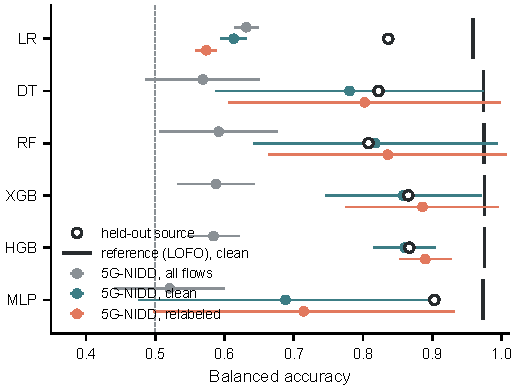
\includegraphics[width=\columnwidth]{figs/fig_transfer}
\caption{Balanced accuracy of detectors trained on \DA{}, on held-out \DA{} (open circles) and on \DB{} (filled, with corrected 95\% interval over 20 splits) for all flows, clean flows, and with the copies relabeled. Vertical bar: the reference trained on \DB{} with each capture file held out, on the clean flows. On consistent labels the tree-based models score as well on \DB{} as on held-out \DA{}, but well below what \DB{} itself allows.}
\label{fig:transfer}
\end{figure}

\emph{A third corpus.} From \DA{} to \DC{} (Table~\ref{tab:third}, 20 splits), balanced accuracy is \RTrCAllBAmin{} to \RTrCAllBAmax{} and ROC-AUC \RTrCAllAUCmin{} to \RTrCAllAUCmax{}; the loss against held-out source data is not significant for any architecture. Inside \DC{}, the same architectures reach \ThRefShRandBAmin{} to \ThRefShRandBAmax{} on a random split and \ThRefShLofoBAmin{} to \ThRefShLofoBAmax{} when the capture file of one attack type is held out. Every architecture detects the SYN flood, which training contained (recall \RCSynMax{} for all six), whereas recall on the ICMP flood is \RCIcmpMin{} to \RCIcmpMax{} and on the PFCP attack, an attack type absent from \DA{}, \RCPfcpMin{} to \RCPfcpMax. Most errors come from the benign traffic of the new site: the false positive rate is \RCFPRmin{} to \RCFPRmax{}, and up to \RCBkgMax{} of the core network's own signaling is flagged. In the reverse direction, models trained on \DB{} reach \RRevABAmin{} to \RRevABAmax{} on \DA{} and \RRevCBAmin{} to \RRevCBAmax{} on \DC{}.

\begin{table*}[t]
\caption{Transfer to the third corpus \DC{} (5G core testbed, NFStream flows with Ethernet and GTP-U bytes removed~\cite{nugraha2025fivegdatasets}): balanced accuracy on held-out source data and on \DC{}, target ROC-AUC, recall per attack type, and the share of the core's own signaling flagged (Bkg.), at $\tau = 0.5$. Mean over 20 splits from \DA{} and 20 from \DB{} (split by capture file).}
\label{tab:third}
\centering
\footnotesize
\begin{tabular}{lccccccccc}
\toprule
 & \multicolumn{7}{c}{Trained on \DA{}} & \multicolumn{2}{c}{Trained on \DB{}} \\
\cmidrule(lr){2-8}\cmidrule(lr){9-10}
Model & Src.\ BA & Tgt.\ BA & AUC & SYN & ICMP & PFCP & Bkg. & Tgt.\ BA & AUC \\
\midrule
LR & 0.837 & 0.742 & 0.800 & 1.00 & 0.10 & 0.00 & 0.27 & 0.552 & 0.708 \\
DT & 0.822 & 0.658 & 0.696 & 1.00 & 1.00 & 0.79 & 0.67 & 0.603 & 0.612 \\
RF & 0.808 & 0.596 & 0.926 & 1.00 & 1.00 & 0.99 & 0.81 & 0.699 & 0.855 \\
XGB & 0.865 & 0.640 & 0.892 & 1.00 & 1.00 & 0.72 & 0.70 & 0.584 & 0.765 \\
HGB & 0.867 & 0.698 & 0.932 & 1.00 & 1.00 & 0.80 & 0.61 & 0.726 & 0.773 \\
MLP & 0.903 & 0.677 & 0.830 & 1.00 & 0.20 & 0.63 & 0.47 & 0.811 & 0.739 \\
\bottomrule
\end{tabular}

\end{table*}

\subsection{What the Gap Consists Of, and Adaptation}
\label{sec:res:gap}

\emph{Byte accounting and separability.} Removing the Ethernet header changed what the shift diagnostics say. A domain classifier (histogram gradient boosting, five-fold cross-validation) tells \DA{} from \DB{} flows with a balanced accuracy of \RDomArgShared{} on the 18 shared columns, but \RDomArgRobust{} on the nine exporter-robust columns, against \RDomOldRobust{} before the correction: the uncorrected header had made the mean packet sizes of the two corpora almost perfectly separable. The robust columns still shift as much as the others ($\bar{W}_1$ of \RWoneArgRobust{} against \RWoneArgNonrobust{} after a quantile map fitted on source data; Fig.~\ref{fig:shift}). The correction did not shrink this shift: most \DB{} flows are UDP and most \DA{} flows TCP, and a 28-byte UDP packet now lies where \DA{} has few packets, whereas the uncorrected 42 bytes had placed it among the 40- to 44-byte TCP packets of \DA{}. The remaining shift is a difference in traffic composition, which no byte accounting removes.

\begin{figure}[t]
\centering
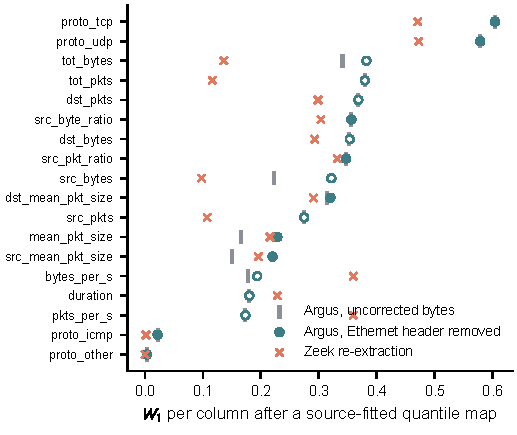
\includegraphics[width=\columnwidth]{figs/fig_shift}
\caption{Covariate shift between \DA{} and \DB{} per shared column: first-order Wasserstein distance after a quantile map fitted on \DA{} training data. Bars: Argus flows before the byte correction; circles: after it (filled: exporter-robust subset); crosses: our Zeek re-extraction of the 5G-NIDD captures. The correction moves the packet-size columns but does not remove the shift.}
\label{fig:shift}
\end{figure}

\emph{A common exporter.} The raw captures of \DB{} are public, so we re-extracted them with Zeek~(version \ZkVersion{}), the exporter family of \DA{}, and labeled each flow by the attack host pairs of its capture file, a rule that reproduces \ZkRuleAgreePct\% of the published labels on the Argus flows. Scored by the same trained models, the clean Zeek flows reach \RZkTreeCleanBAmin{} to \RZkTreeCleanBAmax{} for the tree-based architectures, \RZkTreeCleanDiffMin{} to \RZkTreeCleanDiffMax{} relative to the corrected Argus flows, and the domain classifier separates \DA{} from the Zeek flows as well as from the Argus flows (\RDomZkShared{} on all columns, \RDomZkRobust{} on the robust ones). Our Zeek configuration may differ from the undocumented one behind \DA{} in timeouts or single-packet handling, so this comparison cannot separate traffic composition from exporter configuration.

\emph{Feature subset and adaptation without target labels.} Table~\ref{tab:arms} tests whether other inputs or adaptation methods close the gap. Restricting the models to the nine exporter-robust columns raises held-out source balanced accuracy for five architectures but lowers it for LR (\RArmRobLRSrc{} against \RArmPlainLRSrc). On the clean target flows, XGB and HGB keep their level (\RArmRobXGBClean{} and \RArmRobHGBClean), whereas DT and RF fall to \RArmRobDTClean{} and \RArmRobRFClean: the columns that an exporter moves least are not enough. None of the three adaptation methods that read unlabeled target flows beats the plain tree-based models. Importance weighting changes little (\RArmIwTreeCleanMin{} to \RArmIwTreeCleanMax{} for the tree-based models), because its domain classifier separates the corpora so well that the weights concentrate on \RIwESSmin\% to \RIwESSmax\% of the source flows in effective sample size. CORAL raises the MLP from \RArmPlainMLPClean{} to \RArmCoralMLPClean{} but pushes the target false positive rate of the tree-based models to \RArmCoralTreeFPRmin{} to \RArmCoralTreeFPRmax, as in our first analysis. Domain-adversarial training reaches \RArmDannDANNClean.

\begin{table}[t]
\caption{Transfer from \DA{} to \DB{} under other feature sets and with adaptation, mean over 20 splits, at $\tau = 0.5$. Importance weighting, CORAL, and DANN read unlabeled target flows. Clean: the benign-labeled copies removed; relab.: the copies labeled as attack.}
\label{tab:arms}
\centering
\scriptsize
\setlength{\tabcolsep}{2.6pt}
\begin{tabular}{llccccc}
\toprule
Arm & Model & Src.\ BA & \multicolumn{3}{c}{Target, clean} & Target, relab. \\
\cmidrule(lr){4-6}
 & & & BA & AUC & FPR & BA \\
\midrule
Shared space (18) & LR & 0.837 & 0.613 & 0.796 & 0.061 & 0.574 \\
 & DT & 0.822 & 0.781 & 0.783 & 0.206 & 0.802 \\
 & RF & 0.808 & 0.818 & 0.879 & 0.232 & 0.836 \\
 & XGB & 0.865 & 0.858 & 0.896 & 0.083 & 0.886 \\
 & HGB & 0.867 & 0.860 & 0.888 & 0.064 & 0.890 \\
 & MLP & 0.903 & 0.688 & 0.806 & 0.432 & 0.715 \\
\midrule
Exporter-robust (9) & LR & 0.804 & 0.615 & 0.821 & 0.646 & 0.632 \\
 & DT & 0.883 & 0.616 & 0.633 & 0.546 & 0.647 \\
 & RF & 0.894 & 0.599 & 0.781 & 0.578 & 0.630 \\
 & XGB & 0.925 & 0.835 & 0.847 & 0.076 & 0.870 \\
 & HGB & 0.939 & 0.837 & 0.860 & 0.082 & 0.871 \\
 & MLP & 0.937 & 0.651 & 0.815 & 0.479 & 0.681 \\
\midrule
Importance weighting & LR & 0.696 & 0.624 & 0.789 & 0.533 & 0.630 \\
 & DT & 0.831 & 0.782 & 0.754 & 0.167 & 0.802 \\
 & RF & 0.788 & 0.812 & 0.878 & 0.223 & 0.830 \\
 & XGB & 0.831 & 0.837 & 0.882 & 0.103 & 0.858 \\
 & HGB & 0.814 & 0.740 & 0.863 & 0.220 & 0.768 \\
 & MLP & 0.842 & 0.684 & 0.795 & 0.438 & 0.707 \\
\midrule
CORAL & LR & 0.836 & 0.585 & 0.855 & 0.741 & 0.597 \\
 & DT & 0.818 & 0.539 & 0.543 & 0.794 & 0.546 \\
 & RF & 0.805 & 0.482 & 0.761 & 0.985 & 0.489 \\
 & XGB & 0.903 & 0.539 & 0.736 & 0.766 & 0.560 \\
 & HGB & 0.891 & 0.521 & 0.741 & 0.820 & 0.536 \\
 & MLP & 0.932 & 0.813 & 0.815 & 0.177 & 0.825 \\
\midrule
DANN & DANN & 0.895 & 0.655 & 0.814 & 0.600 & 0.661 \\
\bottomrule
\end{tabular}

\end{table}

\emph{A few labeled target captures.} Labeled data from the target helps far more (Fig.~\ref{fig:labeleff}). Added to the \DA{} training data, a single labeled capture file of \DB{} raises the balanced accuracy of the five nonlinear architectures on the capture files not drawn to \RLeSrcOneNlMin{} to \RLeSrcOneNlMax{} (the MLP from \RLeZeroMLP{} to \RLeSrcOneMLP), close to the leave-one-capture-file-out reference, and eight files to \RLeSrcEightNlMin{} to \RLeSrcEightNlMax. The same capture files alone give only \RLeTgtOneNlMin{} to \RLeTgtOneNlMax{} for one file, so the source data still carries most of what the detectors know. The alert bound takes more data. With the threshold fixed on source data, the six architectures met all three alert conditions in \RLeSrcOneMeet{} of \RLeSrcOneCells{} draws with one labeled file and in \RLeSrcEightMeet{} of \RLeSrcEightCells{} with eight; with eight files, XGB and the MLP met them in every draw, at \RLeSrcEightXGBAlerts{} and \RLeSrcEightMLPAlerts{} false alerts per hour on average and a recall of about \RLeSrcEightXGBRecall.

\begin{figure*}[t]
\centering
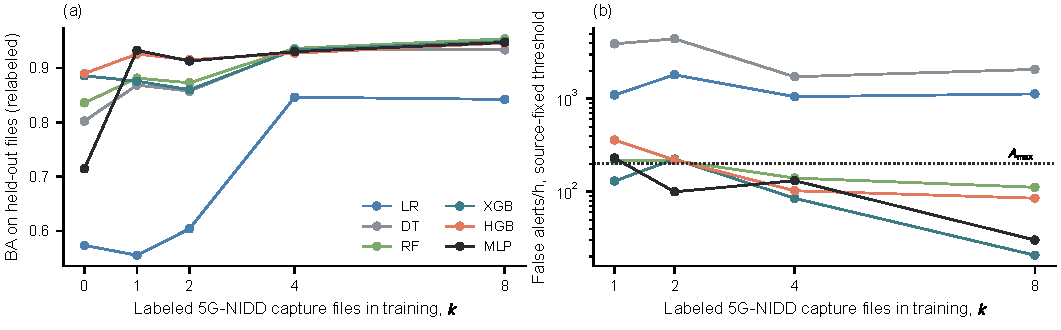
\includegraphics[width=0.92\textwidth]{figs/fig_label_efficient}
\caption{Label-efficient arm: $k$ labeled capture files of \DB{} added to the \DA{} training data (four random draws per $k$; $k = 0$ is the plain transfer of the 20 splits), evaluated on the capture files not drawn, with the copies relabeled as attack. (a) Balanced accuracy; (b) false alerts per hour at the threshold fixed on source data, mean over draws, with the bound $A_{\max}$.}
\label{fig:labeleff}
\end{figure*}

\emph{Size of the source sample.} Repeating the transfer with \RSzNlist{} source flows (\RSzSplits{} splits, five architectures) changed clean target balanced accuracy by at most \RSzMaxChangeClean{} against \NSub{} flows, in no consistent direction, which is within the variation between splits.

